% English version of paper/ja_v2/03_共通の設定.md (2026-11-17).
\section{Data, features, classifiers and settings}\label{sec:setup}

This section describes what the three questions share; settings specific to each question are given at the start of Sects.~\ref{sec:rq1a}--\ref{sec:rq2}.

\subsection{Corpora and four emotions}
We use six corpora that differ in elicitation, recording and annotation as seven groups (Table~\ref{tab:corpora}). IEMOCAP \cite{busso2008iemocap} is split into improvised and scripted groups, because in scripted sessions ten actors read the same lines and a text classifier could succeed by memorising them. The leave-one-corpus-out (LOCO) setting (Sect.~\ref{sec:settings}) uses the four corpora with audio, visual and text (AFEW, the improvised part of IEMOCAP, MOSEI and MELD), and the RQ2 evaluation adds CREMA-D (audio and visual). Labels are mapped to Neutral, Happy, Sad and Angry \cite{ryumina2025}, and utterances of other emotions are not used. In IEMOCAP, happy and excited are merged into Happy and frustration is not mapped to Angry. In MOSEI, an utterance with exactly one emotion of intensity at least 0.5 receives that emotion, one with none receives Neutral, and one with two or more is not used, so MOSEI Neutral is not a neutral rating by annotators.

\begin{table}[t]
\caption{The seven groups. Speaker and utterance counts are after restricting to four emotions, for the single-source and all-source settings; utterance and per-emotion counts are for the audio (WavLM) set, with differing visual or text counts in parentheses. Mod.: modalities. All corpora are in English (RAVDESS: North American English). Counts of the LOCO setting are in Table~\ref{tab:loco}}\label{tab:corpora}
\footnotesize\setlength{\tabcolsep}{3pt}
\begin{tabular}{@{}p{1.75cm}p{2.0cm}p{2.3cm}p{0.95cm}r p{1.75cm}p{1.9cm}@{}}
\toprule
Group & Elicitation & Annotation & Mod. & Speakers & Utterances & N / H / S / A \\
\midrule
AFEW \cite{dhall2012afew,dhall2013emotiw} & Movie acting (partly natural) & Facial-expression category by raters & A, V, T$^{b}$ & 282$^{a}$ & 795 & 207 / 213 / 178 / 197 \\
IEMOCAP impro.\ \cite{busso2008iemocap} & Improvised acting & Plurality of raters' categories & A, V, T & 10 & 2,943 & 1,099 / 947 / 608 / 289 \\
IEMOCAP script.\ \cite{busso2008iemocap} & Scripted acting & Same & A, V, T & 10 & 2,588 (V 2,549) & 609 / 689 / 476 / 814 \\
MOSEI \cite{zadeh2018mosei} & None (opinion monologues) & Crowd intensities of six emotions; our rule & A, V, T & 2,626$^{c}$ & 18,919 (V 18,634) & 8,847 / 6,790 / 1,830 / 1,452 \\
MELD \cite{poria2019meld} & TV-series acting & Majority of raters' categories & A, V, T & 283 & 11,343 (V 11,308, T 11,344) & 6,430 / 2,305 / 1,002 / 1,606 \\
CREMA-D \cite{cao2014cremad} & Instructed acting, 12 sentences & Acted emotion; crowd ratings & A, V & 91 & 4,900 (V 4,899) & 1,087 / 1,271 / 1,271 / 1,271 \\
RAVDESS \cite{livingstone2018ravdess} & Instructed acting, 2 sentences & Acted emotion; validated by raters & A & 24 & 672 & 96 / 192 / 192 / 192 \\
\botrule
\end{tabular}
\footnotetext{$^{a}$Number of actor names. $^{b}$AFEW text features come from Whisper large-v3 transcripts (790 utterances) and were made after the single-source and all-source computations, which therefore do not use them. $^{c}$Number of channels or video IDs (Sect.~\ref{sec:split}). The two IEMOCAP groups share the same ten actors. Concatenated features are built only from utterances that have all of the concatenated modalities}
\end{table}

\subsection{Speaker-independent splits}\label{sec:split}
In every setting, no speaker appears on both the training and the evaluation side (speaker-independent), and official splits are not used. MOSEI has no speaker annotation, so the YouTube channel (known for 1,122 of 3,225 videos) or otherwise the video ID serves as the speaker; the same person may therefore appear on both sides in different videos. In the LOCO setting, aliases of the same MELD actor are merged, speaker names that do not identify a single voice are dropped, and AFEW utterances linked by actor or by movie form one cluster.

\subsection{Features and classifiers}
Features are encoder outputs averaged within each utterance; no encoder is fine-tuned on our corpora. Audio: 16 kHz waveforms (first 60 s) are fed to WavLM-large \cite{chen2022wavlm} and the last layer is averaged over time (1,024 dimensions); in the single-source setting we also use the last layer of HuBERT-large \cite{hsu2021}. Visual: the largest face is cropped with YOLOv8n-face\footnote{https://github.com/derronqi/yolov8-face (GPL-3.0), trained on WIDER FACE \cite{yang2016}.} from 5--6 frames per second (for IEMOCAP, the half of the screen showing the speaker), and the 512-dimensional outputs of a ResNet-50 expression model \cite{ryumina2022} are averaged over frames. Text: transcripts are fed to RoBERTa-base \cite{liu2019roberta} and the last layer is averaged over tokens (768 dimensions); human transcripts are used for IEMOCAP, MOSEI and MELD and Whisper large-v3 \cite{radford2023whisper} outputs for AFEW. RAVDESS and CREMA-D have no text features because their sentences are fixed, and RAVDESS has no visual features. Classifiers on concatenated features of two or three modalities (AV, VT, AT, AVT) are also built. We write A for audio, V for visual and T for text.

Every classifier is a multinomial logistic regression trained on per-dimension standardised features. With $n$ training utterances and $n_k$ of emotion $k$, utterances of emotion $k$ are weighted by $\omega_k=n/(4n_k)$ so that the emotion proportions of the training data do not enter the classifier. In the single-source setting, the classifier weights carry an L2 penalty with inverse strength $C$ and the intercepts are unpenalised; $C\in\{0.01,0.1,1,10\}$ is chosen by speaker-split three-fold cross-validation (the merged classifier uses the $C$ of the source-only classifier of the same repetition). In the all-source and LOCO settings, the classifier weights and intercepts are pulled towards a classifier built from the sources (the \emph{anchor}) with strengths $C'$ and $C_b$, chosen with source groups or corpora as provisional targets (Sect.~\ref{sec:settings}). Test labels are never used to choose hyperparameters.

\subsection{Three settings}\label{sec:settings}
The three settings differ in how labelled source utterances are used (Fig.~\ref{fig:settings}).
\begin{itemize}
\item \textbf{Single-source setting} (Sect.~\ref{sec:rq1a}): for each ordered pair of groups (target, source), all utterances of one source group and K target labels are trained together (merged classifier); classifiers trained on the source only and on the K target labels only are also built. The test set is one of five speaker folds of the target, and repetitions 0--9 change the folds and the test fold.
\item \textbf{All-source setting} (Sect.~\ref{sec:rq1a}): a classifier built from all groups except the target is the anchor and is retrained on the K target labels (K-label baseline), with K = 0, 5 and 25.
\item \textbf{LOCO setting} (Sects.~\ref{sec:rq1b} and \ref{sec:rq2}): one of AFEW, IEMOCAP (improvised), MOSEI and MELD is the target and the other three are sources. The mean of the weights and intercepts of the three source classifiers is the anchor, and the classifier retrained from it on the K target labels is the \emph{K-label baseline} (at K = 0, the anchor itself, i.e., source only). The test set is one of five folds that keep each cluster within one fold (one session for IEMOCAP; utterance and cluster counts in Table~\ref{tab:loco}), and the remaining target utterances are the \emph{candidates}; K labels per emotion are drawn from the candidates and no other candidate labels are used. Values are averaged over 50 repetitions (5 folds $\times$ 10 draws of the K labels; 5 repetitions for K = 0).
\end{itemize}

\begin{figure}[t]
\centering
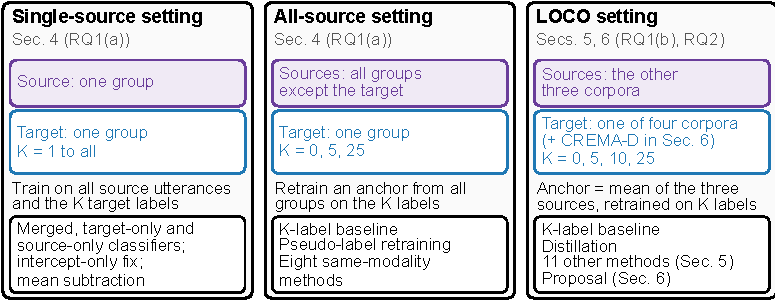
\includegraphics[width=\textwidth]{figures/fig_v2_settings_en.pdf}
\caption{The three settings. The single-source and all-source settings serve RQ1(a) (Sect.~\ref{sec:rq1a}); the LOCO setting serves RQ1(b) (Sect.~\ref{sec:rq1b}) and RQ2 (Sect.~\ref{sec:rq2}). Groups: IEMOCAP improvised and scripted, MOSEI, MELD, AFEW, CREMA-D and RAVDESS}\label{fig:settings}
\end{figure}

LOCO hyperparameters were selected on runs in which each of the three corpora other than the evaluation target served in turn as a provisional target (with the remaining two corpora as sources; 3 corpora $\times$ 5 folds $\times$ 2 seeds = 30 repetitions) and fixed, and the evaluation target was computed once with the fixed settings (evaluation run). We call each provisional-target computation an \emph{episode}. Outputs inspected before and during the evaluation run are stated in Sects.~\ref{sec:distill} and \ref{sec:hp}.

\begin{table}[t]
\caption{Utterances of the LOCO setting (utterances with all of audio, visual and text; CREMA-D: audio and visual). ``Effective'' is the effective number of clusters, $(\sum_g n_g)^2/\sum_g n_g^2$ for cluster sizes $n_g$}\label{tab:loco}
\footnotesize\setlength{\tabcolsep}{4pt}
\begin{tabular}{@{}lrllr@{}}
\toprule
Corpus & Utterances & N / H / S / A & Clusters & Effective \\
\midrule
AFEW & 790 & 205 / 211 / 177 / 197 & 51 (actor/movie links) & 14.99 \\
IEMOCAP (improvised) & 2,943 & 1,099 / 947 / 608 / 289 & 5 (sessions) & 4.91 \\
MOSEI & 18,634 & 8,637 / 6,734 / 1,814 / 1,449 & 2,614 (channels/videos) & 783.22 \\
MELD & 11,267 & 6,383 / 2,283 / 999 / 1,602 & 272 (speakers) & 8.59 \\
CREMA-D & 4,899 & 1,087 / 1,271 / 1,270 / 1,271 & 91 (speakers) & 90.98 \\
\botrule
\end{tabular}
\end{table}

\subsection{Metric and intervals}
The main metric is UAR (unweighted average recall over emotions), whose chance level with four emotions is 25\%. Overall accuracy (weighted accuracy) is not reported because it depends on the share of Neutral, which differs across corpora. UAR and its differences are in percentage points, and the difference A $-$ B between two classifiers is called the \emph{gain}; each section states A and B. All intervals are 95\% intervals without multiple-comparison correction; they reflect the sampling of test speakers (clusters for MOSEI and the LOCO setting) and of the K labels, not the choice of source corpora, training utterances, methods or hyperparameters. Intervals of the single-source and all-source settings are described in Sects.~\ref{sec:rq1a-single} and \ref{sec:rq1a-all}. For the LOCO setting, the variance of a cluster jackknife (cluster resampling for MOSEI and CREMA-D) is added to the variance over K-label draws; because inference with few clusters is anti-conservative \cite{cameron2008}, jackknife $t$ intervals are used for corpora with fewer than 20 effective test clusters. Conditions of the same corpus that differ only in K share test utterances and nested K labels and are not independent. We write that UAR \emph{rose} or \emph{fell} only when the 95\% interval of the difference lies above or below zero, and write ``higher in point estimates'' otherwise.
